\chapter{Decoders}\label{sec:surface_decoders}
\section{The optimal decoder}\label{sec:optimal_decoder}
\section{Minimum Weight Perfect Matching}\label{sec:MWPMdecoder}

\subsection{Quasiparticle picture}
The processes of error detection and correction can alternatively be presented in the \emph{quasiparticle picture}, where the anticommuting stabilizer measurements act like excitations on the lattice, which behave like the quasiparticles \emph{anyons}. A single error creates a pair of anyons, and a chain of errors causes movement of the anyon on the lattice. A pair of anyons can also annihilate each other when two error chains merge. The correction of errors can thus be viewed of movement of the correction chains until all anyons are annihilated. The quasiparticle picture removes the distracting underlying lattice from the problem, and decoding becomes simply identifying the right pairing between anyons to minimize the chance of a logical error.
\tikzstyle{rednode}=[circle, fill=red!50, minimum size=4]
\tikzstyle{bluenode}=[circle, fill=cyan!50, minimum size=4]
\tikzstyle{redline}=[red!50, line width = 2]
\tikzstyle{blueline}=[cyan!50, line width = 2]
\tikzstyle{legend}=[anchor=west, font=\small]

\newcommand{\drawquasigrid}{
  \draw[step=.4cm, opacity=.25] (0,0) grid (4,4);
  \draw (0,0) rectangle (4,4);
  \node[rednode] (N1) at (0.5,0.4) {};
  \node[rednode] (N2) at (2,0.7) {};
  \node[rednode] (N3) at (2.5,1.2) {};
  \node[rednode] (N4) at (3.6,1) {};
  \node[rednode] (N5) at (0.75,2.1) {};
  \node[rednode] (N6) at (1.95,1.8) {};
  \node[bluenode] (N7) at (1.6, 3.4) {};
  \node[bluenode] (N8) at (2.7, 3.5) {};
  \node[bluenode] (N9) at (3.2, 2.2) {};
  \node[bluenode] (N10) at (3.1, 0.6) {};
  \draw[blueline] (N1) to[in=170, out=20] (N2);
  \draw[blueline] (N3) to[in=180, out=-10] (N4);
  \draw[blueline] (N5) to[in=170, out=-20] (N6);
  \draw[redline] (N7) to[in=160, out=15] (N8);
  \draw[redline] (N9) to[in=90, out=250] (N10);
}
\begin{figure}
    \centering
    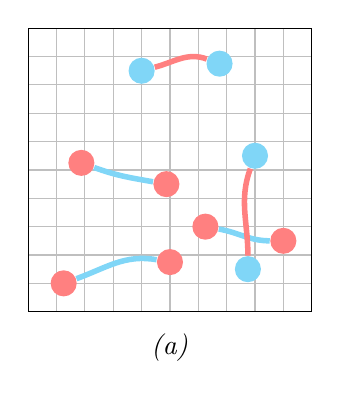
\begin{tikzpicture}[scale=0.9]
      \drawquasigrid
      \node at (2, -.5) {\emph{(a)}};
    \end{tikzpicture}
    \hspace{.3cm}
    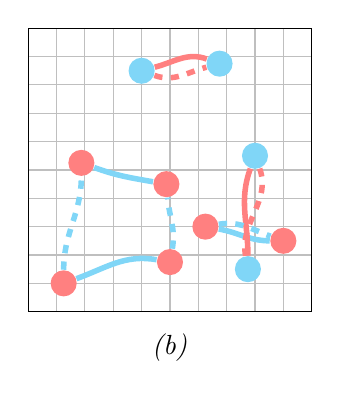
\begin{tikzpicture}[scale=0.9]
      \drawquasigrid
      \draw[dashed, blueline] (N1) to[out=90, in=270] (N5);
      \draw[dashed, blueline] (N2) to[out=80, in=275] (N6);
      \draw[dashed, blueline] (N3) to[out=10, in=160] (N4);
      \draw[dashed, redline] (N7) to[out=-20, in=195] (N8);
      \draw[dashed, redline] (N9) to[out=290, in=100] (N10);
      \node at (2, -.5) {\emph{(b)}};
    \end{tikzpicture}
    \hspace{.3cm}
    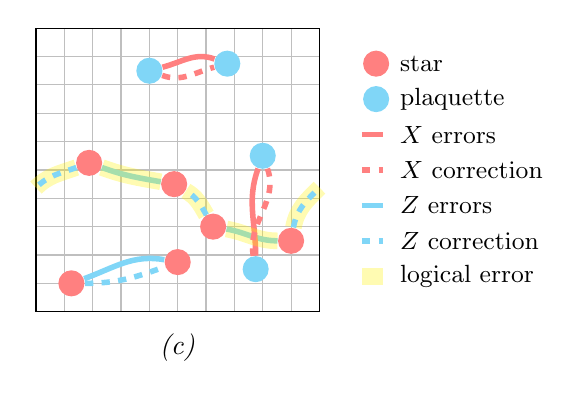
\begin{tikzpicture}[scale=0.9]
      \drawquasigrid
      \draw[yellow, line width=6, opacity=.3] (N3) to[in=180, out=-10] (N4);
      \draw[yellow, line width=6, opacity=.3] (N5) to[in=170, out=-20] (N6);
      \draw[yellow, line width=6, opacity=.3] (N3) to[out=120, in=-30] (N6);
      \draw[yellow, line width=6, opacity=.3] (N5) to[out=200, in=45] (0, 1.75);
      \draw[yellow, line width=6, opacity=.3] (N4) to[out=80, in=225] (4, 1.75);
      \draw[dashed, blueline] (N1) to[out=0, in=200] (N2);
      \draw[dashed, blueline] (N3) to[out=120, in=-30] (N6);
      \draw[dashed, blueline] (N5) to[out=200, in=45] (0, 1.75);
      \draw[dashed, blueline] (N4) to[out=80, in=225] (4, 1.75);
      \draw[dashed, redline] (N7) to[out=-20, in=195] (N8);
      \draw[dashed, redline] (N9) to[out=290, in=100] (N10);
      \node at (2, -.5) {\emph{(c)}};


      \node[rednode] at (4.8, 3.5){};
      \node[bluenode] at (4.8,3){};
      \draw[redline] (4.6,2.5) -- +(0.3,0);
      \draw[redline, dashed] (4.6,2) -- +(0.3,0);
      \draw[blueline] (4.6,1.5) -- +(0.3,0);
      \draw[blueline, dashed] (4.6,1) -- +(0.3,0);
      \draw[yellow, line width=6, opacity=.3] (4.6,.5) -- +(0.3,0);
      \path (5,3.5) node[legend] {star} ++(0,-.5) node[legend] {plaquette} ++(0,-.5) node[legend] {$X$ errors} ++(0,-.5) node[legend] {$X$ correction} ++(0,-.5) node[legend] {$Z$ errors} ++(0,-.5) node[legend] {$Z$ correction} ++(0,-.5) node[legend] {logical error} ;
    \end{tikzpicture}
    \caption{The quasiparticle picture of stabilizer measurements. Anticommuting stabilizers behave as anyons (circles), where a chain of errors (lines) creates a pair of anyons. Figure (b) shows a successful decoding of (a). Figure (c) shows a pairing that resulted in a correction operator that is in a different class as the error operator, which acquires a logical error. (Figure inspired by \cite{naomi})}\label{fig:quasiparticle}
  \end{figure}
  
Figure \ref{fig:quasiparticle}a shows the quasiparticle representation of the errors suffered in Figure \ref{sf:fig_degenerate}a, which has suffered Z (blue lines) and X errors (red lines). The corresponding anyons can either be of the star type (red circle) or plaquette type (blue circle). Figure \ref{fig:quasiparticle}b shows a successful decoding. Note that here not all pairs are correctly identified, but the resulting loop still is in the same class of operators. In figure \ref{fig:quasiparticle}c the correction has failed as the resulting loop in the correction is in a difference class compared to the error. As the loop still commutes with the stabilizer, no error can be detected, but the encoded qubit has acquired a logical error.


\section{Union-Find}\label{sec:UFdecoder}

The Union-Find decoder is a new fast decoding algorithm for topological codes to correct for Pauli errors, erasure errors, and the combination of both errors. The worst-case complexity of the algorithm is $\m{O}(n\alpha(n))$, where $n$ is the number of physical qubits and $\alpha$ is the inverse of Ackermann's function, which is very slowly growing, and is proven that $a(n)\leq 3$ for any practical amount of qubits.

Many types of decoding algorithms have been developed for the surface code, including the optimal decoder and the MWPM-decoder. Most of these decoders run at best in polynomial time, which is often considered efficient, but in practice even quadratic or cubic complexity is likely too slow to correct errors faster than they accumulate in a quantum device. Furthermore, any speed-up of the decoder will indirectly lead to a reduction of the noise strength, as a shorter time between two rounds of correction allows for fewer errors to appear. To this end, a new decoding algorithm named the \emph{Peeling decoder} has been developed that can solve errors over the erasure channel with a linear time complexity. The \emph{Union-Find} decoder is an extensions that additionally solves for Pauli errors. We will explore both algorithms in the coming sections and perform analyses on their complexities. 

\subsection{The Peeling decoder}
he Peeling decoder acquired its name by the nature of its behavior of sequentially \emph{peeling} from some tree of qubit-edges until the correction operator is left \cite{delfosse2017linear}. The scope of this decoder is limited to \emph{erasure} errors, or errors suffered through the erasure channel. Recall from equation \eqref{qec:eq:erasure} that in an erasure, each qubit is erased from the system independently with probability $p_E$. Such a loss can be detected and the missing qubit is replaced by a totally mixed state of equation \eqref{qec:eq:mixstate}, which can be interpreted as the original state that suffers from a Pauli error $I$, $X$, $Y$ or $Z$ chosen uniformly at random.
\begin{theorem}\label{the:independentxy}
  For erasure noise of equation \eqref{qec:eq:erasure}, where a qubit is erased and replaced with a totally mixed state equivalent to a qubit that suffers from uniformly chosen $\{I,X,Y,Z\}$, the primal and dual lattices of the surface code can be decoded independently from each other. 
\end{theorem}
\begin{proof}
  Pauli $X$ errors exclusively trigger nontrivial star operator measurement on the vertices of the primal lattice. Pauli $Z$ errors exclusively trigger trigger nontrivial plaquette measurements on the vertices of the dual lattice, or faces of the primal lattice. Recall from section \ref{sec:toricgraph} that a graph $G(V,E,F)$ can be separated into sub-graphs $G_{V}(V,E_V)$ and $G_{F}(F,E_F)$. An uniformly distributed $\{I,X,Y,Z\}$ on $G(V,E,F)$ is hence equivalent to uniformly distributed $\{I,X\}$ and $\{I,Z\}$ that simultaneously and separately apply to $G_{V}$ and $G_{F}$, respectively, since $\{I,X\} \otimes \{I,Z\}=\{I,X,Y,Z\}$. 
\end{proof}
\begin{definition}\label{def:erasure}
  Let the subset of qubits that suffer an erasure error (equation \eqref{qec:eq:erasure}) on a lattice $G(V,E)$ be denoted by $\gls{erasure}\subseteq E$. Edges in $\m{E}$ are replaced by uniformly distributed $\{I,X\}$ for the primal lattice (and $\{I,Z\}$ for the dual lattice). Let the set of edges that suffer an Pauli error due to this replacement by $P_\m{E}\subseteq \m{E}$. 
\end{definition}
\begin{definition}\label{def:pauliprod}
  The \emph{Pauli product} of a set of edges $\tilde{E}$ is the defined as the product of Pauli operators on each of the edges in the set
  \begin{equation}\label{eq:pauliprod}
    \gls{pauliproduct}(\tilde{E}) = \prod_{e\in \tilde{E}} \hat{P}_e,
  \end{equation}
  where the Pauli operator $\hat{P}$ corresponds to $X$ if $\tilde{E}\subseteq E_v$ and otherwise $Z$ when $\tilde{E}\subseteq E_f$. 
\end{definition}

\subsubsection{Decoder process}
In this section, we will only consider the sub-graph $G_{V}(V,E_V)$ and denote it simply by $G(V,E)$. We describe the decoding process of an erasure $\m{E}$ with errors on $P_\m{E}$. Error detection is performed in the same way as Pauli errors; by measuring the set of stabilizer operators on vertices $V$, which returns a set of nontrivial syndrome measurements $\sigma \subseteq V$. The decoder of an erasure error is thus provided with the extra information $\m{E}$ on top of the nontrivial measurements $\sigma$. The decoding process of sub-graph $G_{F}(F,E_F)$ is equivalent to the process of $G_{V}(V,E_V)$.
\begin{lemma}\label{lem:peelinguni}
  For an erasure $\m{E} \subseteq E$ whose qubits are reinitiated with uniformly distributed Pauli errors resulting in errors on $P_\m{E}$, and a measured syndrome $\sigma$, any error $\tilde{P}_\m{E} \subseteq \m{E}$ that produces $\sigma$ in a measurement is the most likely set of errors. 
\end{lemma}
\begin{proof}
  % For the coset $\tilde{P}_\m{E}\cdot S$, where $\tilde{P}_\m{E}$ is some Pauli error caused by an erasure and $S$ is a set of stabilizers that act trivially on the codespace, the most likely configuration is the one that maximizes probability $\mathbb{P}(\tilde{P}_\m{E}\cdot S|\m{E},\sigma)$, where $\m{E}$ and $\sigma$ are known. This probability is proportional to $|\tilde{P}_\m{E}\cdot S \cap\m{E}|$. But since all qubits in $\m{E}$ suffer a Pauli error and this error is uniformly distributed, all configurations of $\tilde{P}_\m{E}$ have equal probability. 
  In the absence of Pauli errors, all edges with some error $P$ must lie inside $\m{E}$. Therefore, for any measured syndrome $\sigma$, the path of errors must also be in the erasure, which can be denoted by $\tilde{P}_\m{E} \subseteq \m{E}$. Since all errors in $\m{E}$ are uniformly distributed, any set of edges with errors $\tilde{P}_\m{E}$ with syndrome $\sigma$ is the most likely set. 
\end{proof}

For this reason, if the correction $\hat{C}=\n{P}(\tilde{P}_\m{E})$ is applied to the lattice, the resulting decoder is a \emph{maximum likelihood decoder}. In order to find $\hat{C}$, the objective is not try to find paths within $\m{E}$ that pair the syndrome vertices of $\sigma$, but rather try to recursively shrink the set of edges on which a decision is to be made. 
\begin{definition}\label{def:boundaryofedges}
  The vertex boundary or support of a set of edges $\gls{boundary}(\tilde{E})$ denotes the set of vertices $\tilde{V}$ that supports all edges $e\in \tilde{E}$.
\end{definition}
\begin{definition}\label{def:forest}
  A spanning forest $F_{\tilde{E}}$ is a maximal subset of edges of $\tilde{E}$ that contains no cycles and $\mathscr{B}(F_{\tilde{E}}) = \mathscr{B}(\tilde{E})$.
\end{definition}
The first step  is to produce $\gls{forest}$ inside $\m{E}$, where all syndrome vertices $\sigma$ are included in the support per definition \ref{def:forest}. Hence if $\m{E}$ is a connected graph, then $F_\m{E}$ is a connected \emph{acyclic} graph. Such a forest can be found in linear time by either a depth-first search of the $\m{E}$. Next, the decoder further reduces the size of the spanning forest $F_\m{E}$ by sequentially peeling edges from the tree, while constructing the correction set $\gls{correctionset}\subseteq F_\m{E}$, initiated as an empty set. The decoder loops over all edges in $F_\m{E}$, each time picking a \emph{leaf} edge $e = \{u,v\}$, connected to the forest by only one vertex $v$, removing the leaf edge from $F_\m{E}$. If the so-called \emph{pendant} vertex $u$ belong to the set of nontrivial syndrome measurements $\sigma$, remove $u$ from $\sigma$, add $e$ to $\m{C}$, and \emph{flip} the vertex $v$ in $\sigma$, such that $v$ is added to $\sigma$ if $v \notin \sigma$, and removed from $\sigma$ if $v\in\sigma$.  If $u\notin\sigma$, the edge $e$ is simply removed from $F_\m{E}$ (see algorithm \ref{algo:peel}). On account of these rules, edges on a branch that had a syndrome vertex as a leaf will continuously be added to $\m{C}$ until it encounters another syndrome vertex, creating a correction path between a syndrome pair. The forest is peeled until there are not edges in $F_\m{E}$ and $\hat{C}=\n{P}(\m{C})$.
\begin{algo}[algotitle=Peeling decoder (adapted from \cite{delfosse2017linear}), label=algo:peel]
  \begin{algorithm}[H]
    \KwData{A graph $G = (V,E)$, an erasure $\m{E} \subseteq E$ and syndrome $\sigma \subseteq V$}
    \KwResult{Correction $\hat{C}$}
    \BlankLine
    construct a spanning forest $F_\m{E} \subseteq\m{E}$\;
    initialize $\m{C} = {\emptyset}$\;
    \While{$F_\m{E} \neq \emptyset$}{
    pick a leaf edge $e = {u,v}$ with pendant vertex $u$, remove $e$ from $F_\m{E}$ \;
    \If{$u \in \sigma$}{
      add $e$ to $\m{C}$, remove $u$ from $\sigma$ and flip $v$ in $\sigma$}
    \Else{do nothing}
    }
    \KwRet{$\n{P}(\m{C})$, see equation \eqref{eq:pauliprod}}
  \end{algorithm}
\end{algo}
\tikzset{
  anyon/.style={circle, fill=OrangeRed, minimum size=.2cm, inner sep=0},
  erasure/.style={NavyBlue, very thick},
  correction/.style={Green, very thick},
  description/.style={align=#1, text width=4cm},
  description/.default={left},
  error/.style={text=black, pos=0.5}
  }

\begin{figure}
  \centering
  \begin{tikzpicture}[on grid, scale=0.8]
    \node at (0,4) {a)};
    \draw[step=1cm,gray,thin] (0.1,0.1) grid (3.9,3.9);
    \draw[erasure] (1,1) -- (2,1) node[error]{$X$} -- (3,1) -- (3,2) -- (2,2) -- (1,2) -- cycle node[error]{$X$};
    \draw[erasure] (1,2) -- (1,3) -- (2,3) node[error]{$X$} -- (2,2);
    \node[description={center}] at (2, -.5) {initial state};

    \begin{scope}[shift={(6,0)}]
      \node at (0,4) {b)};
      \draw[step=1cm,gray,thin] (0.1,0.1) grid (3.9,3.9);
      \draw[erasure] (1,1) -- (2,1) node[anyon]{} -- (3,1) -- (3,2) -- (2,2) -- (1,2) node[anyon] (a) {} -- cycle;
      \draw[erasure] (a) -- (1,3) node[anyon]{} -- (2,3) node[anyon]{}-- (2,2);
      \node[description={center}] at (2, -.5) {identify syndrome};
    \end{scope}

    \begin{scope}[shift={(12,-.5)}]
      \draw[thin] (0,4) -- ++(.5,0) ++(.5,0) node[anchor=west]{normal edge};
      \draw[thin] (0,3) -- ++(.5,0) node[error]{$X$} ++(.5,0) node[anchor=west]{Pauli error};
      \draw[erasure] (0,2) -- ++(.5,0) ++(.5,0) node[anchor=west, text=black]{erased edge};
      \draw[thin] (0,1) -- ++(.5,0) node[anyon,pos=.5]{} ++(.5,0) node[anchor=west]{syndrome};
      \draw[correction] (0,0)   -- ++(.5,0) ++(.5,0) node[anchor=west,text=black]{correction edge};
    \end{scope}

    \begin{scope}[shift={(0,-6)}]
      \node at (0,4) {c)};
      \draw[step=1cm,gray,thin] (0.1,0.1) grid (3.9,3.9);
      \draw[erasure] (1,3) node[anyon]{} -- (2,3) node[anyon]{} -- (2,2) -- (1,2) node[anyon]{} -- (1,1) -- (2,1) node[anyon]{} -- (3,1) -- (3,2);
      \node[description={center}] at (2, -.5) {construct $F_{\varepsilon}$};
    \end{scope}

    \begin{scope}[shift={(6,-6)}]
      \node at (0,4) {d)};
      \draw[step=1cm,gray,thin] (0.1,0.1) grid (3.9,3.9);
      \draw[erasure] (1,3) node[anyon]{} -- (2,3) node[anyon]{} -- (2,2) -- (1,2) node[anyon]{} -- (1,1) -- (2,1) node[anyon](a){};
      \draw[erasure, dashed] (a) -- (3,1) node[pos=0, below, text=black]{$v$} node[pos=0.5, above]{$e$} node[pos=1, below, text=black]{$u$};
      \node[description={center}] at (2, -.5) {peel $e=(u,v), u \notin \sigma$};
    \end{scope}

    \begin{scope}[shift={(12,-6)}]
      \node at (0,4) {e)};
      \draw[step=1cm,gray,thin] (0.1,0.1) grid (3.9,3.9);
      \draw[erasure] (1,3) node[anyon]{} -- (2,3) node[anyon]{} -- (2,2) -- (1,2) node[anyon]{} -- (1,1);
      \draw[erasure, dashed] (1,1) node[below, text=black]{$v$} -- (2,1) node[anyon]{} node[pos=0.5, above]{$e$} node[below, text=black]{$u$};
      \node[description={center}] at (2, -.5) {peel $e=(u,v), u \in \sigma$};
    \end{scope}

    \begin{scope}[shift={(0,-12)}]
      \node at (0,4) {f)};
      \draw[step=1cm,gray,thin] (0.1,0.1) grid (3.9,3.9);
      \draw[erasure] (1,3) node[anyon]{} -- (2,3) node[anyon]{} --  (2,2) -- (1,2) node[anyon]{} -- (1,1) node[anyon](a){};
      \draw[correction] (a) node[below, text=black]{$v$} -- (2,1) node[pos=0.5, above]{$e$} node[below, text=black]{$u$};
      \node[description={center}] at (2, -.5) {flip $u,v$, add $e$ to $C$};
    \end{scope}

    \begin{scope}[shift={(6,-12)}]
      \node at (0,4) {g)};
      \draw[step=1cm,gray,thin] (0.1,0.1) grid (3.9,3.9);
      \draw[correction] (1,3) -- (2,3) node[error]{$X$} (2,1) -- (1,1) node[error]{$X$} -- (1,2) node[error]{$X$};
      \node[description={center}] at (2, -.5) {apply correction set $C$};
    \end{scope}

    \begin{scope}[shift={(12,-12)}]
      \node at (0,4) {h)};
      \draw[step=1cm,gray,thin] (0.1,0.1) grid (3.9,3.9);
      \node[description={center}] at (2, -.5) {end state};
    \end{scope}
  \end{tikzpicture}
  \caption{Schematic representation of the Peeling decoder. On an erasure $\m{E}\subset E$ (a), there may be some Pauli errors $P\subset \m{E}$ that anticommutes with some stabilizer measurements (b) that is identified as the syndrome $\sigma$. The first step is to construct a spanning forest $F_\m{E}\subset \m{E}$, a fully connected acyclic graph. Next the decoder sequentially removes leaf edges $e=(u,v)$ from the forest that connect to the forest via only one vertex $v$. If $u\in\sigma$ (e), remove $u$ from $\sigma$, flip $v$ in $\sigma$ and the edge $e$ is added to the correction set $C$ (f). If $u \notin \sigma$, move on the the next leaf. After applying the correction set $C$, all errors on the lattice commutes with the stabilizers, potentially solving the error (h).}
\end{figure}

\subsubsection{Decoder validity}
The spanning forest $F_\m{E}$ can be constructed in linear time. Also, the loop over the forest can be operated in linear if the list of leaves is pre-computed and updated during the loop. Thus the Peeling decoder has a linear time complexity in the size of the erasure $\m{O}(\abs{\m{E}})$ and therefore also in the number of qubits $\m{O}(n)$. The structure of the forest $F_\m{E}$ is dependent on the root vertex from which the depth-first search is started, and proof is required that any forest of $\m{E}$ is valid. Also, we show that for all forests, the peeling process returns the same correction.

\begin{lemma}\label{lem:anyforest}
  For any choice of $F_\m{E}$, there exists a subset $\m{C}\subseteq F_\m{E}$ such that $\mathscr{P}(\m{C})$ corrects the syndrome set $\sigma$.
\end{lemma}
\begin{proof}
  There exists a subset of edges $\m{C} = \{e_1,e_2,...\} \subseteq F_\m{E}$ such that $\mathscr{P}(\m{C})$ has a syndrome $\sigma$. By the definition of the forest $F_\m{E}$, adding another edge $e' \in F_\m{E} \vartriangle \m{E}$ creates a cycle $\gamma' \subseteq F_\m{E} \cup \{e'\}$, where $\vartriangle$ denotes the symmetric difference between two sets. Now $\m{C}$ can be replaced by $\m{C}'=\m{C}\vartriangle\gamma'$ whose Pauli product $\mathscr{P}(\m{C}')$ has the same syndrome $\sigma$, as $\vartriangle$ augments the matching path between syndromes within $\gamma'$. Now, any edge $e_r\in \gamma' \vartriangle \m{C}'$ can be removed from $F_\m{E} \cup \{e'\}$ to create a new forest $F_\m{E}'=F_\m{E} \cup \{e_i\}\setminus e_r$. For any cycle that exists from larger than 3 elements, $e_r$ must exist. Thus the Pauli product of subset $\m{C}' \subseteq F_\m{E}'\subseteq \m{E}$ is also a valid error with syndrome $\sigma$, and $\mathscr{P}(\m{C}')$ corrects $\sigma$. This can be done any number of times, thus every $F_\m{E}$ is valid.   
\end{proof}
\begin{lemma}\label{lem:peelingfe}
  For each forest $F_\m{E}$, the outcome $\m{C}$ after peeling is unique and independent from the order of peeling. 
\end{lemma}
\begin{proof}
   If there exists two subsets $\m{C}\subseteq F_\m{E}$ and $\m{C}' \subseteq F_\m{E}$, such that $\n{P}(\m{C})$ and $\n{P}(\m{C}')$ corrects $\sigma$, then $\mathscr{P}(\m{C})\mathscr{P}(\m{C}')$ commutes with the stabilizer. This means that either $\m{C}\vartriangle\m{C}'$ is a cycle or $\m{C}=\m{C}'$. Since $F_\m{E}$ has no cycles it means that $\m{C}$ must be unique within $F_\m{E}$.
\end{proof}

Per lemmas \ref{lem:anyforest} and \ref{lem:peelingfe}, for some error $P_\m{E}$ on erasure $\m{E}$, the Peeling decoder will always output some correction $\n{P}(\m{C})$ such that $\n{P}(\m{C})\n{P}(P_\m{E})$ commutes with the stabilizer. This correction is also the most likely correction per lemma \ref{lem:peelinguni}. Finally, we will prove that this is true for any erasure $\m{E}\subseteq E$. 
\begin{theorem}\label{the:anyevenparity}
  For any connected erasure $\m{E}\subseteq E$ with pauli error on $P_\m{E}$, if the parity of the number syndrome vertices within the graph is even, applying the Peeling decoder (algorithm \ref{algo:peel}) will produce a valid correction $\n{P}(\m{C})$.
\end{theorem}
\begin{proof}
  Consider a spanning forest $F_\m{E}$ containing $n_\sigma$ syndrome vertices. The forest is being stripped by the Peeling decoder on the leaf edge $e = (u,v)$, where the vertex $v$ is the pendant vertex. If $u\notin\sigma$, $e$ is simply removed from $F_\m{E}$ and $n_\sigma$ is unaltered. If $u\in\sigma$, $u$ is removed from $\sigma$ such that $n_\sigma'= n_\sigma -1$. Vertex $v$ is now flipped in $\sigma$, meaning that if $v\in\sigma$, it is removed and $n_\sigma'= n_\sigma -2$, or if  $v\notin\sigma$, it is added and $n_\sigma'= n_\sigma$. After peeling it must be that $n_\sigma=0$, from which follows that all erasures with \emph{even} parity can be solved. 
\end{proof}

\begin{definition}\label{def:cluster}
  A cluster $C$ is a subset of an erasure $\m{E}$, such that the edges of $C$ form a connected graph. The parity of $C$ is the number of syndromes in its vertex boundary. 
  \begin{equation}\label{eq:clusterparity}
    \text{parity}(C) = \abs{\{v\in \sigma \cap \bound(C)\}}
  \end{equation}
\end{definition}
\begin{lemma}\label{lem:singlecluster}
  An edge can only belong to a single cluster. A vertex can only be in the vertex boundary of a single cluster $\mathscr{B}(C)$. 
\end{lemma}
\begin{proof}
  If there exists some edge $e$ that belongs to two clusters $C_i, C_j$, they are connected via $e$. Per definition \ref{def:cluster} clusters $C_i, C_j$ must be a single cluster. The same is true for some vertex $v$ that belongs to both $\mathscr{B}(C_i)$ and $\mathscr{B}(C_j)$. 
\end{proof}
Given a graph $G(E,V)$ that is subjected to pure pure erasure noise, $\m{E}$ may not be a single subset of connected edges, but rather many connected subsets, or clusters, denoted by $\{C_1, C_2,...\}$. For each cluster $C_i$, all syndromes caused by errors on $P_{C_i}$ must be supported by $\bound(C_i)$. Since every cluster must be strictly disjoint per lemma \ref{lem:singlecluster}, the parity for each $C_i$ must therefore be even, and $C_i$ can be decoded individually per theorem \ref{the:anyevenparity}. Here, each $C_i$ a forest is made and peeled. This is why erasure noise is the scope of the Peeling decoder. As other types of noise are added, modifications to the Peeling decoder are needed, as we will see later. 
\begin{theorem}
  The Peeling decoder (algorithm \ref{algo:peel}) is a linear-time maximum likelihood decoder for erasures up to $d-1$ qubits, where $d$ is the minimum distance of the code. 
\end{theorem}
\begin{proof}
  If the erasure $\m{C}$ does not support a subset of edges that is equivalent to some logical operator $L=\mathscr{P}(\tilde{E})|\tilde{E}\subseteq\m{E}$, the product of the error and correction $CP_\m{E}$ cannot lead to a logical error, as $\m{C}\subseteq \m{E}$. Furthermore, on account of lemmas \ref{lem:peelinguni}, \ref{lem:anyforest} and \ref{lem:peelingfe}, any correction set $\m{C}\subseteq F_\m{E}$ is the most likely correction. Thus for any erasure pattern up to $d-1$ qubits, the Peeling decoder is a linear-time maximum likelihood decoder. 
\end{proof}

\subsubsection{Bounded surfaces}
For bounded surfaces such as the planar code (sec \ref{sec:surface_planar}), the peeling decoder needs some small alterations. Recall that the graph of the primal lattice is now denoted by $G = (V_\iota\cup V_{\delta} \cup V_{\omega}, E_\iota \cup E_{\delta})$. Syndrome measurements on such a graph are only supported by $\sigma \subseteq V_\iota\cup V_\omega$, as $V_\delta$ are \emph{open} vertices that only exist to support boundary edges $E_\delta$, and do not refer to some stabilizer generator or physical measurement. The missing information on $V_\delta$ makes it impossible to apply the pendant vertex rule at these vertices. To ensure that the peeling algorithm does not become stuck, we add the restriction for the pendant vertex $u \notin V_\delta$. Furthermore, the construction of the forest $F_\m{E}$ requires an additional alteration.
\begin{lemma}
  Two vertices $u,v$ within a forest $F_\m{E}$ that satisfy $u\in V_\delta, v \in V_\delta$ is equivalent to a cycle in $F_\m{E}$. 
\end{lemma}
\begin{proof}
  If there are an even number of vertices in a forest $F_\m{E}$ that are supported by $V_\delta$, it means that there are a number of unique paths within $F_\m{E}$ that lead from a element of $V_\delta$ to another element of $V_\delta$. Such a path is equivalent to some $\delta$-operators and commutes with the stabilizer. Hence, it cannot be caused by some detected error which anticommutes with the stabilizer.
\end{proof}

Due to this, we ensure that each forest $F_\m{E}$ can only support a maximum of 1 element of $V_\delta$. The forests are grown starting from vertices of the set $V_\delta$, and the algorithm is completed by a depth-first search same as before with the additional requirement. Note that now for every cluster, more than one connected acyclic forests may be formed, dependent on the number edges connected to the boundary. But as all forests $\{F_1, F_2,...\}$ that are subsets of the same cluster are disjoint, each edge is peeled only once and every forest can be peeled independently per lemma \ref{lem:anyforest}. With these extra rules in mind, we present the pseudo-code of the Peeling decoder for bounded surfaces in algorithm \ref{algo:peelbound}. 

\begin{algo}[algotitle=Peeling decoder for bounded surfaces (adapted from \cite{delfosse2017linear}), label=algo:peelbound]
  \begin{algorithm}[H]
    \KwData{A graph $G = (V_{\iota\omega}\cup V_\delta,E)$, an erasure $\m{E} \subseteq E$ and syndrome $\sigma \subseteq V_{\iota\omega}$}
    \KwResult{Correction $\hat{C}$}
    \BlankLine
    construct a spanning forest $F_\m{E}\subseteq\m{E}$ with seed $V_\delta$\;
    initialize $\m{C} = {\emptyset}$\;
    \While{$F_\m{E} \neq \emptyset$}{
    pick a leaf edge $e = {u,v}$ with pendant vertex $u\notin V_\delta$, remove $e$ from $F_\m{E}$ \;
    \If{$u \in \sigma$}{
      add $e$ to $\m{C}$, remove $u$ from $\sigma$ and flip $v$ in $\sigma$}
    \Else{do nothing}
    }
    \KwRet{$\n{P}(\m{C})$, see equation \eqref{eq:pauliprod}}
  \end{algorithm}
\end{algo}

\begin{figure}
    \centering
    \begin{tikzpicture}[on grid, scale=0.8]
      \node at (-.5,4) {\emph{(a)}};
      \draw[step=1cm,gray,thin] (0.1,0) grid (3.9,4);
      \draw[erasure] (0.1,1) -- (1,1)  -- (2,1)  node[error]{$X$} -- (2,2) -- (2,3) -- (1,3)  -- (1,2) node[error]{$X$}  -- (0.1,2)  node[error]{$X$} (1,1) -- (1,2) -- (2,2);
      \draw[erasure] (3.9,4) -- (3,4)  node[error]{$X$} -- (3,3)  -- (3,2)  node[error]{$X$}  -- (3.9,2) (2,3) -- (3,3) -- (3.9,3);
      \node[description={center}] at (2, -.5) {initial state};
  
      \begin{scope}[shift={(6,0)}]
        \node at (-.5,4) {\emph{(b)}};
        \draw[step=1cm,gray,thin] (0.1,0) grid (3.9,4);
        \draw[erasure] (0.1,1) -- (1,1) node[anyon]{} -- (2,1) node[anyon]{} -- (2,2) -- (2,3) -- (1,3) node[anyon]{} -- (1,2)  -- (0.1,2) (1,1) -- (1,2) -- (2,2);
        \draw[erasure] (3.9,4) -- (3,4) node[anyon]{} -- (3,3) node[anyon]{} -- (3,2) node[anyon]{}  -- (3.9,2) (2,3) -- (3,3) -- (3.9,3);
        \node[description={center}] at (2, -.5) {identify syndrome};
      \end{scope}
  
      \begin{scope}[shift={(12,-.5)}]
        \draw[thin] (0,4) -- ++(.5,0) ++(.5,0) node[anchor=west]{normal edge};
        \draw[thin] (0,3) -- ++(.5,0) node[error]{$X$} ++(.5,0) node[anchor=west]{Pauli error};
        \draw[erasure] (0,2) -- ++(.5,0) ++(.5,0) node[anchor=west, text=black]{erased edge};
        \draw[thin] (0,1) -- ++(.5,0) node[anyon,pos=.5]{} ++(.5,0) node[anchor=west]{syndrome};
        \draw[correction] (0,0)   -- ++(.5,0) ++(.5,0) node[anchor=west,text=black]{correction edge};
      \end{scope}

      \begin{scope}[shift={(0,-6)}]
        \node at (-.5,4) {\emph{(c)}};
        \draw[step=1cm,gray,thin] (0.1,0) grid (3.9,4);
        \draw[erasure] (0.1, 2) -- (1,2) -- (1,1) node[anyon]{} -- (2,1) node[anyon]{} -- (2,2) -- (2,3) -- (1,3) node[anyon]{};
        \draw[erasure] (3.9,4) -- (3,4) node[anyon]{} -- (3,3) node[anyon]{} -- (3,2) node[anyon]{};
        \node[description={center}] at (2, -.5) {construct $\m{T}_\m{R}$};
      \end{scope}

      \begin{scope}[shift={(6,-6)}]
        \node at (-.5,4) {\emph{(d)}};
        \draw[step=1cm,gray,thin] (0.1,0) grid (3.9,4);
        \draw[correction] (0.1, 2) -- (1,2) node[error]{$X$} -- (1,1) node[error]{$X$} (2,1)  -- (2,2) node[error]{$X$} -- (2,3) node[error]{$X$} -- (1,3) node[error]{$X$};
        \draw[correction] (3.9,4) -- (3,4) node[error]{$X$} (3,3) -- (3,2) node[error]{$X$};
        \node[description={center}] at (2, -.5) {apply correction $\n{P}(\m{C})$};
      \end{scope}

      \begin{scope}[shift={(12,-6)}]
        \node at (-.5,4) {\emph{(e)}};
        \draw[step=1cm,gray,thin] (0.1,0) grid (3.9,4);
        \path (1,1) -- (2,1) node[error]{$X$} -- (2,2) node[error]{$X$} -- (2,3) node[error]{$X$} -- (1,3) node[error]{$X$} -- (1,2) node[error]{$X$} -- (1,1) node[error]{$X$};
        \node[description={center}] at (2, -.5) {end state};
      \end{scope}

    \end{tikzpicture}
    \caption{Schematic visualization of the Peeling decoder on a surface with boundaries. On an erasure $\m{R}\subset \m{E}$ (a), there may be some Pauli errors $\m{E}_\m{R} \subset \m{R}$ that anticommute with some stabilizer measurements (b) that is identified as the syndrome $\sigma$. (c) The forest $\m{T}_\m{R}$ now has the extra constriction that it can only support single elements of $\m{V}_\delta$, the open vertices, and peeling is only allowed on pendant vertices $v\notin \m{V}_\delta$. (d) After peeling, the correction $\n{P}(\m{C})$ is outputted and can be applied to correct error. (e) The end state is now a cycle of errors, which commutes with the stabilizer. This is not a feature of the Peeling decoder, but is just an example.}
  \end{figure}


% To keep track of the vertices of a cluster, it will be represented as a \emph{cluster tree}, where an arbitrary vertex of the cluster will be the root, and any other vertex will be a child of the root. Whenever an edge $(u,v)$ is fully grown, we will need to traverse the trees of the two vertices $u$ and $v$, and check whether they have the same root; whether they belong to the same cluster. If not, a merge is initiated by making the root of smaller cluster a child of the bigger cluster. These functions, \codefunc{find} and \codefunc{union} respectively, are part of the Union-Find algorithm (not to be confused with the Union-Find decoder) \cite{tarjan1975efficiency}.

% Within the Union-Find algorithm, two features ensure that the complexity of the algorithm is not quadratic. 1). With \textbf{path compression}, as we traverse a tree from child to parent until we reach the root, we make sure that each vertex encountered that we have encountered along the way is pointed directly to the root. This doubles the cost of the \codefunc{find}, but speeds up any future call to any vertex on the traversed path. 2). With \textbf{weighted union}, we make sure to always make the smaller tree a child of the bigger tree. This ensures that the overall length of the path to the root stays minimal. In order to make this happen, we just need to store the size of the tree at the root.

\subsection{Union-Find decoder}
The Union-Find decoder \cite{delfosse2017almost} is a modification of the Peeling decoder that utilizes the Union-Find data structure \cite{tarjan1975efficiency} to additionally solve for Pauli errors, on top of erasure errors. In this section, we will first describe why a modification is needed, then how the Union-Find data structure is applied, and finally move on the the algorithm itself and analyze its complexity. 

The Peeling decoder solves exclusively for erasure errors. To be able to compare with the MWPM decoder, or any other type of decoders, Pauli noise must be included. To this end, we use the independent noise model of equations \ref{qec:eq:bitflip} and \ref{qec:eq:phaseflip}. This means that we can again consider the primal and dual lattices separately, as $X$ errors exclusively trigger nontrivial star operator measurements on the vertices of the primal lattice, and $Z$ errors exclusively trigger nontrivial plaquette measurements on vertices of the dual lattice. These noise channels introduce extra Pauli errors $P_p$ such that not all Pauli errors are in the erasures $P\not\subseteq \m{E}$, where $P = P_p\triangle P_\m{E}$. This means also that not all syndromes are in the boundary of the erasure $\sigma \not\subseteq \mathscr{B}(\m{E})$ (definition \ref{def:boundaryofedges}), and odd parity clusters can occur. Per theorem \ref{the:anyevenparity}, the Peeling decoder cannot solve for these errors.

To this end, we construct an altered erasure $\bar{\m{E}}$ that contains only even-parity clusters can be constructed from the syndrome $\sigma$ in a pre-processing step that is dubbed \emph{syndrome validation}. The validated erasure $\bar{\m{E}}$ is compatible with the peeling decoder. To do this, we sequentially grow the clusters with an odd parity on the boundaries of the clusters. When two odd parity clusters meet, the merged cluster will have a even parity, and can now be solved by the peeling decoder. 
\begin{proposition}
  The Peeling decoder can be altered to additionally solve for Pauli errors by a pre-processing step that initializes some altered erasure $\bar{E}$, such that theorem \ref{the:anyevenparity} is satisfied, after which the Peeling decoder can proceed as before. 
\end{proposition}
\begin{figure}[h]
  \centering
  \begin{tikzpicture}
    \node[draw, circle, OrangeRed, fill=OrangeRed!50!white, line width=1, text=black] (s1) at (0,1.5) {$\sigma$};
    \node[draw, circle, NavyBlue, fill=NavyBlue!50!white, line width =1, text=black] (e1) at (0,.5) {$\m{E}$};
    \node[draw, circle, OrangeRed, fill=OrangeRed!50!white, line width=1, text=black] (s2) at (5,1.5) {$\sigma$};
    \node[draw, circle, NavyBlue, fill=NavyBlue!50!white, line width =1, text=black] (e2) at (5,.5) {$\bar{\m{E}}$};
    \draw[OrangeRed, line width = 1] (s2) -- +(-1,0);
    \draw[NavyBlue, line width = 1] (e2) -- +(-1,0);
    \draw[OrangeRed, line width = 1, -latex]  (s1) -- +(1,0);
    \draw[OrangeRed, line width = 1, -latex] (s2) -- +(1,0);
    \draw[NavyBlue, line width = 1, -latex] (e1) -- +(1,0);
    \draw[NavyBlue, line width = 1, -latex] (e2) -- +(1,0);
    \node[draw, circle, Green, fill=Green!50!white, line width=1, text=black] (c) at (10,1) {$C$};
    \draw[Green, line width = 1, latex-] (c) -- +(-1,0);
    \node[left=0 of s1, align=right] {syndrome};
    \node[left=0 of e1, align=right] {erasure};
    \node[right=0 of c, align=left] {correction};
    \draw[line width=1] (1,0) rectangle +(3,2) (6,0) rectangle ++(3,2);
    \node[text width = 2cm, align=center] at (2.5,1) {\emph{Syndrome validation}};
    \node[text width = 2cm, align=center] at (7.5,1) {\emph{Peeling decoder}};
  \end{tikzpicture}
  \caption{Stages of decoding of the Union-Find decoder. A pre-processing step that is called \emph{syndrome validation} is added to the Peeling decoder such that an altered erasure $\bar{\m{E}}$ is constructed that satisfies theorem \ref{the:anyevenparity}, where all erasures have an even number of syndromes. (Figure inspired by \cite{delfosse2017almost})} 
  \label{fig:ufstages}
\end{figure}
Per lemma \ref{lem:singlecluster}, an edge can only be in a single cluster $C$ and a vertex in a single cluster boundary $\mathscr{B}(C)$. The merge of two clusters thus requires the update of the parent cluster of at least one set of vertices and edges. The challenge is to efficiently store this cluster index value such that the update complexity after each merge is minimized. This is done via the Union-Find data structure.

\subsubsection{Application of the Union-Find data structure}
The Union-Find data structure, also known as the \emph{disjoint-set} data structure \cite{tarjan1975efficiency}, consist of two functions for manipulating a set of elements partitioned into a number of disjoint subsets, and a set of rules for these manipulations. In the context of the surface code, the vertices $v\in V$ are the elements and each disjoint set is the set over vertices that support a cluster $\mathscr{B}(C)$ (definitions \ref{def:boundaryofedges}, \ref{def:cluster}). It is redundant to additionally store the sets $C$ for edges, as it lemma \ref{lem:singlecluster} implies that if a vertex $v\in \mathscr{B}(C)$, that all edges support by $v$ satisfy $e \in C$. 

More specifically, we'll be using the disjoint-set tree implementation; each cluster is denoted by a tree, where each element or vertex points to its parent vertex. The function \codefunc{Find}$(v)$ is performed by following the parent pointers to the root $r_v$ of the tree, which is the representative element of the cluster. The function \codefunc{Union}$(r_u,r_v)$ links the trees of vertices $u$ and $v$ by making one of the roots a child of another. We apply \emph{union by rank} and \emph{path compression} to ensure that the complexity is $\m{O}(n\alpha(n))$, where $\alpha(n)$ is the inverse of Ackermann's function and $n$ denotes the system size or number of vertices in $V$. For all practical purposes, $\alpha(n)\leq 4$. The Union-Find data structure, its tree implementation, the \emph{union by rank} and \emph{path compression} rules are all elaborately covered in appendix \ref{ap:unionfind}. Here, we also make a full analysis of its $\m{O}(n\alpha(n))$ complexity based on \cite{kozen1992design}. The Ackermann's function and its inverse are detailed in appendix \ref{ap:ackermann}

Note that while the nodes in the tree are equivalent to vertices $v \in V$, parent pointers in the disjoint-set tree structure are \emph{not} equivalent to edges $e\in E$. The edge set $E$ with its erasure subset $\m{E}\subseteq E$ and subsequently cluster $C\subseteq \m{E}$ and forest $F_C\subseteq C$ are related to physical qubits and the lattice structure of the surface code, whereas edges of the tree $\bound(C)$ exists to point towards the representative element at the root.

\subsubsection{Union-Find decoder data structure}
We define in this section what it means to grow a cluster. For a cluster defined by disjoint-set tree of vertices $\bound(C)$, an iteration of growth means to add another layer of vertices that lie on the other boundary of the tree. To this end, we can view the edges $\delta C$ for which only one connected vertex in $\bound(C)$ as paths lead to the new vertices to be added to the tree. 
\begin{equation}
  \delta C = \{e=(u,v)\in C | u \in \bound(C), v \notin \bound(C)\}
\end{equation}
To grow a cluster, we thus traverse paths and add all vertices $\{v | (u,v) \in \delta C\}$ to the tree, by making it point toward the root $r_u$ in the tree. We denote this as the growth of edges $\delta C$. Note that every single-vertex addition to the tree can be viewed as an union event. If $v$ does not belong to another cluster, the addition is an union event between the tree of $\bound(C)$ and a single-element tree $\{v\}$. If $v$ does belong to another cluster with tree $\bound(C')$, it is an union event between two trees. We thus always apply $\codefunc{Find}(u)$ and $\codefunc{Find}(v)$ to find the respective roots $r_u, r_v$. If $r_u\neq r_v$, $\codefunc{Union}(r_u, r_v)$ returns the merged tree. 

For two vertices $u,v$ that belong to different odd clusters and connected by $(u,v)$, where $(u,v)\in\delta C_u, (u,v) \in \delta C_v$, a round of growth where both clusters are grown would mean that the path of $(u,v)$ is considered twice. This does not make sense, as in the second traversal o $(u,v)$, both vertices already belong to the same cluster. To this end, we only traverse the path an half-edge length per round of growth. In the case such as above, both traversals from vertices $u$ and $v$ on edge $(u,v)$ cover a half-edge and meet in the middle. The state of how many times a path $e$ is traversed is tracked by a variable dubbed the \emph{support} of an edge $\codefunc{support}[e]$, which can take on values $\{0,1,2\}$; $0$ for \emph{not grown}, $1$ for\emph{half-grown} and $2$ for \emph{fully grown}. Growing an edge means to increase the value of $\codefunc{support}[e]$ by $1$, and to merge the cluster if $\codefunc{support}[e]=2$. 

For the pre-processing step of syndrome validation, we thus needs to 1) store the clusters as disjoint-set trees, 2) store for each cluster the list of boundary edges $\delta C$ and 3) store some table \codefunc{support} for the growth state of all edges. 

\subsubsection{Syndrome validation}
In each round of growth at time $t$, there may be many clusters $C_{i,t}$ grown. If clusters are immediately merged within the same time step $t$ if some boundary edge $e\in \delta C$ reaches $\codefunc{support}[e]=2$, it is not possible to track which clusters have completed their growth and which have not. To this end, \codefunc{Union}'s are applied at the end of each round. 

We initiate a round of growth at time $t$ by collecting a list $\m{L} = \{C_{0,t}, C_{1,t}, ...\}$ of odd syndrome parity clusters. Cluster are grown by growing the edges $e \in \delta C_{i,t} \forall \delta C_{i,t} \in \m{L}$, which is done by $\codefunc{support}[e] = \codefunc{support}[e] +1$. Add all edges with $\codefunc{support}[e]=2$ to a fusion list $\m{F}_t$. After all clusters are grown, for each edge $e=(u,v) \in \m{F}_t$, apply $r_u\codefunc{Find}(u)$ and $r_v\codefunc{Find}(v)$. If $r_u\neq r_v$, the trees of both clusters are merged by $\codefunc{Union}(r_u,r_v)$. At time same time, we find new boundaries $\delta C_{i,t+1}$ which are supported by the newly added vertices $v$ and merge the new boundary lists $\delta C_{u,t+1}$ and $\delta C_{v,t+1}$ during $\codefunc{Union}(r_u,r_v)$. We remove all even cluster from $\m{L}$ and the process can be repeated until $\m{L}=\emptyset$. 



\paragraph{Data structure}
Now it is clear what information is exactly needed to grow the clusters using the Union-Find algorithm. We will need to store the cluster in a sort of cluster-tree. At the root of each tree we store the size and parity of that cluster in order to facilitate weighted union and to select the odd clusters. We will need to store the state of each edge (empty, half-grown, or fully grown) in a table called \codeword{support}. And we need to keep track of the boundary of each cluster in a \codeword{boundary} list.

\paragraph{The routine}
The full routine of the Union-Find decoder as originally described (\cite{delfosse2017almost}, Algorithm 2) is listed in Algorithm \ref{algo:uf}. In line 1-2, we initialize the data structures, and a list of odd cluster roots $\m{L}$. We will loop over this list until it is empty, or that there are no more odd clusters left.

In each growth iteration, we will need to keep track of which clusters have merged onto one, therefore the fusion list $\m{F}$ is initialized in line 4. We loop over all the edges from the \codeword{boundary} of the clusters from $\m{L}$ in line 5, and grow each edge by an half-edge in \codeword{support}. If an edge is fully grown, it is added to $\m{F}$.

For each edge $(u,v)$ in $\m{F}$, we need to check whether the neighboring vertices belong to different clusters, and merge these clusters if they do. This is done using the Union-Find algorithm in line 6. We call \codefunc{find(u)} and \codefunc{find(v)} to find the cluster roots of the vertices. If they do not have the same root, we make one cluster the child of another by \codefunc{union(u,v)}. Note that this does not only merge two existing clusters, also new vertices, which have themselves as their roots, are added to the cluster this way. We also need to combine the boundary lists of the two clusters.

Finally, we need to update the elements in the cluster list $\m{L}$. First, we replace each element $u$ with its potential new cluster root \codefunc{find(u)} in line 7. We can avoid creating duplicate elements by maintaining an extra look-up table that keeps track of the elements $\m{L}$ at the beginning of each round of growth. In line 8, we update the \codeword{boundary} lists of all the clusters in $\m{L}$, and in line 9, even clusters are removed from the list, preparing it for the next round of growth.

\begin{algo}[algotitle=Union-Find decoder \cite{delfosse2017almost}, label=algo:uf]
  \begin{algorithm}[H]
    \KwData{A graph $G = (V,E)$, an erasure $\m{E} \subseteq E$ and syndrome $\sigma \subseteq V$}
    \KwResult{A grown erasure $\m{E}'$ such that each cluster $\gamma \subseteq \m{E}$ is even}
    \BlankLine
    initialize cluster-trees, support and boundary lists for all clusters \;
    initialize list of odd cluster roots $\m{L}$\;
    \While{$\m{L} \neq \emptyset$}{
    initialize fusion list $\m{F}$ \;
    for all $u \in \m{L}$, grow all edges in the boundary list of cluster $C_u$ by a half-edge in support. If the edge is fully grow, add to fusion list $\m{F}$ \;
    for all $e={u,v} \in \m{F}$, if \emph{find($u$)} $\neq$ \emph{find($v$)}, then apply \emph{union($u,v$)}, append boundary list\;
    for all $u \in \m{L}$, replace $u$ with \emph{find($u$)} without creating duplicate elements\;
    for all $u \in \m{L}$, update the boundary list\;
    remove even clusters from $\m{L}$\;
    }
    run peeling decoder with grown erasure $\m{E}'$
  \end{algorithm}
\end{algo}

\subsubsection{Time complexity of the Union-Find decoder}

